\chapter{Implementation}
\label{implementation}

Until now we have described the bootware in a generic context because it should work with various different SWfMSs.
But for the implementation we will have to work with a specific system, which in our case is the SimTech SWfMS.
\autoref{image:generic} shows the bootware being used together with the SimTech SWfMS.
It also shows the components as one of three types: specific, generic, and adapted.
The specific components, shown in black, are those components that belong to a specific SWfMS.
In our case these are the SimTech Modeler at the bottom left and the SimTech ODE (and other components that were omitted in this figure) in the center.
On the other hand we have the generic components, shown in white.
These are components that are build to be generic and can be used in all kinds of environments.
In our case these are the local and remote bootwares and their plugins, as well as the provisioning manager and the ESB (here Apache Service Mix) and various repositories and registries.
The specific and the generic components have to work together, but there should be no need to make huge modifications to either one to do so.
Therefore, we need adapter components in some places, which are shown in gray in \autoref{image:generic}.
They are responsible for gluing together specific and generic components where necessary and should be the only components that have to be modified or created from scratch to fit to a specific environment.
In our case this is the bootware plugin, an implementation of the bootware adapter described in \autoref{design:modeler_integration}, loaded in the SimTech Modeler on the bottom left.
There also is an adapter component between the SimTech ODE and Apache Service Mix, which is not shown here.

\begin{figure}[!htbp]
	\centering
	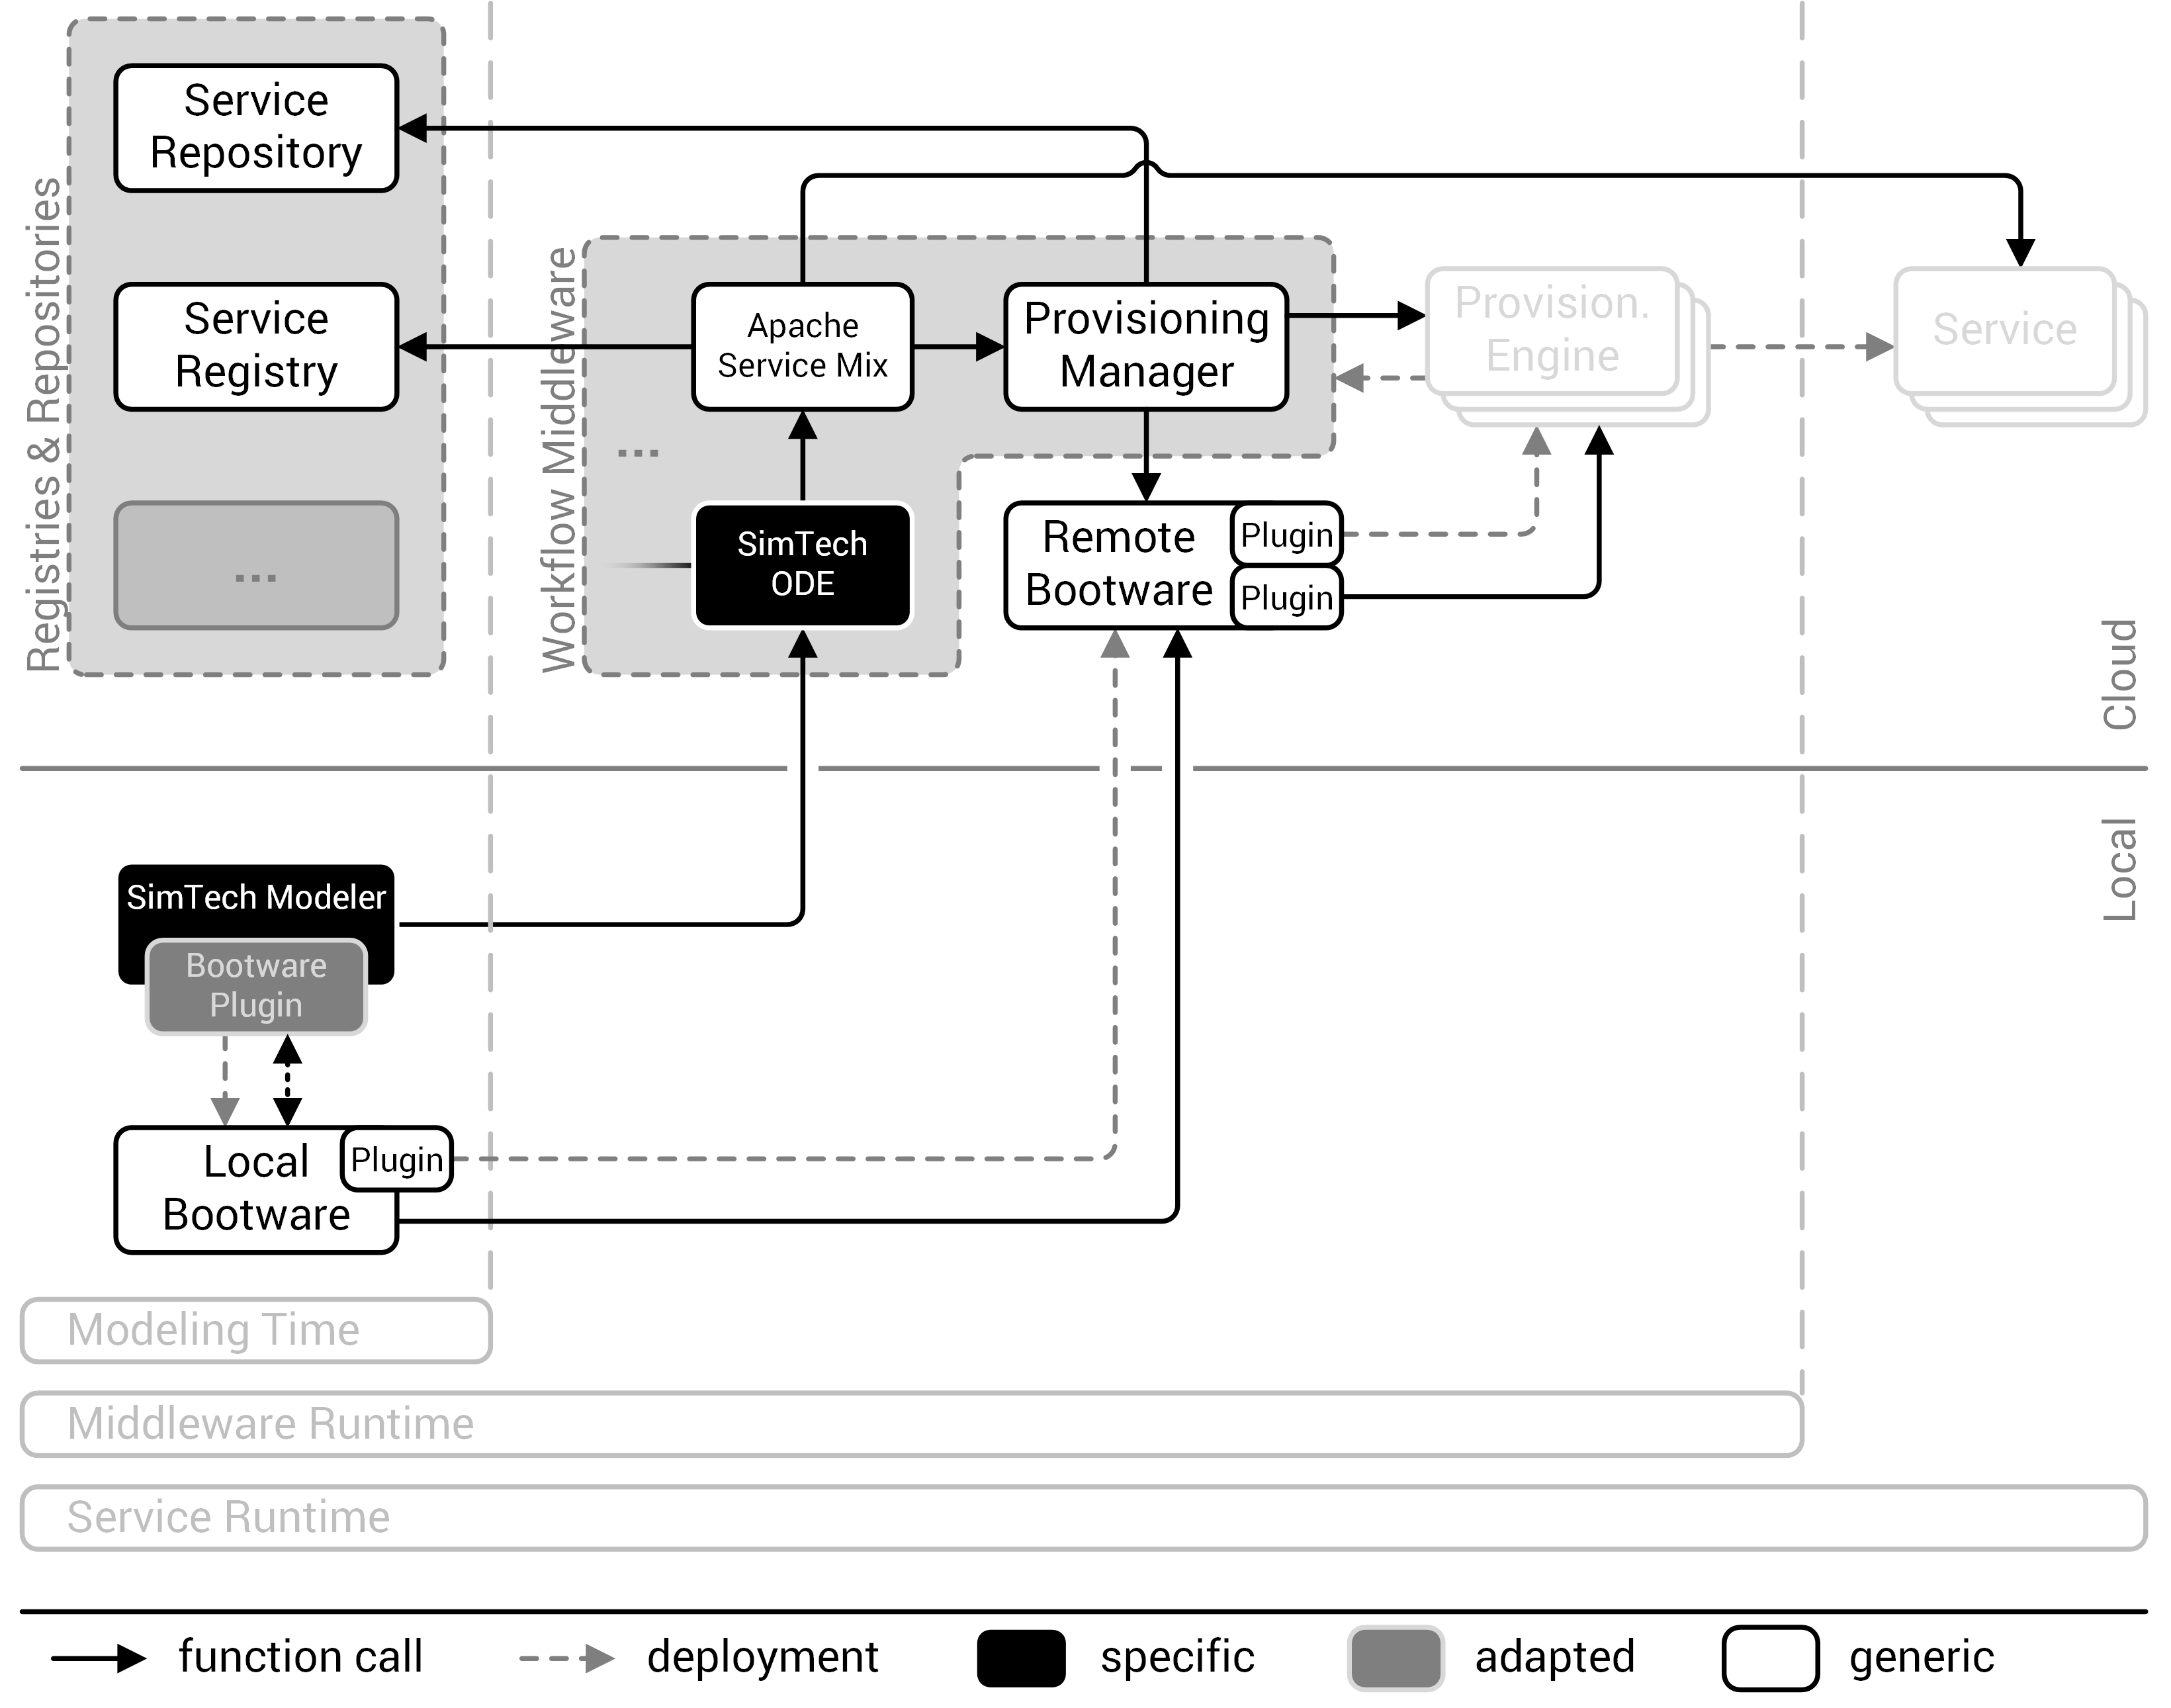
\includegraphics[resolution=600]{implementation/assets/generic}
	\caption{Specific and generic components and adapters.}
	\label{image:generic}
\end{figure}

For the implementation of this diploma thesis we will have to create the generic local and remote bootware components and their plugins, as well as the bootware plugin, which will be specific to the SimTech Modeler.
In the rest of the chapter we present details on the implementation of the bootware components.
First, we describe the implementation of the bootware plugin.
Next, we select specific frameworks and libraries that allow us to implement the architecture we developed in \autoref{design}.
Then, we present detailed descriptions of the implementation of some parts of the local and remote bootware and some plugins.


\section{Modeler Integration}
\label{implementation:modeler_integration}

In this section we describe the integration between the SimTech SWfMS and the bootware.
Currently, what happens is that if a workflow is is ready and should be executed, the user clicks on a button in the SimTech Modeler and the workflow is deployed and executed on the SimTech SWfMS.
Now we have to find a way to integrate the bootware into this process.
We described this as a generic bootware adapter in \autoref{design:modeler_integration}, but now we need an actual implementation of this adapter, which wil be specific to the SimTech Modeler
The button is realized by an Eclipse plugin that adds SimTech specific functionality to the Modeler (which is based on Eclipse).
We therefore also have to create some kind of Eclipse plugin to hook into this process.
We call it the bootware plugin.
There are two scenarios how we could go about this.

We could extend the existing plugin with the functionality that we need for the bootware.
In this case, we would always load the bootware extensions in the Modeler, even if we don't use the bootware at all.
We could also use a feature called extension points.
Eclipse plugins can declare extensions points, which allow other plugins to extend or customize parts of the plugin\footnote{\url{http://wiki.eclipse.org/FAQ_What_are_extensions_and_extension_points\%3F}}.
We could define an extension point in the already existing eclipse plugin and create a second plugin which implements this extension point.
This way we can separate the bootware functionality from the other SimTech extensions and keep the changes to the existing plugin to a minimum.
If a user doesn't need the bootware functionality, they don't have to load the bootware plugin and the SimTech plugin will continue to function as before.

The second scenario looks preferable to the first one, so this is what we are going to do.
We modify the already existing Eclipse plugin with an extension point that is triggered at the beginning of the existing deployment process.
If the bootware plugin is loaded into the Modeler, it will implement this extension point and set up the SimTech SWfMS before the already existing deployment code continues.
If it is not loaded, nothing new will happen and the existing deployment code will be executed like before.
The bootware plugin can also add additional extension to the modeler, for example a configuration dialog for setting up the context or a view that shows progress messages from the bootstrapping process.

\section{Bootware Core Library}

We have seen in \autoref{design:flow} and \autoref{design:finalarch} that the local and remote bootware have some common functionality.
It would make sense to implement these components in such a way that they can share this common functionality.
This would avoid code duplication and make changes to common functionality easier.
Therefore, we introduce the bootware core library, which will encapsulate the common functionality of both bootware components.

\begin{figure}[!htbp]
	\centering
	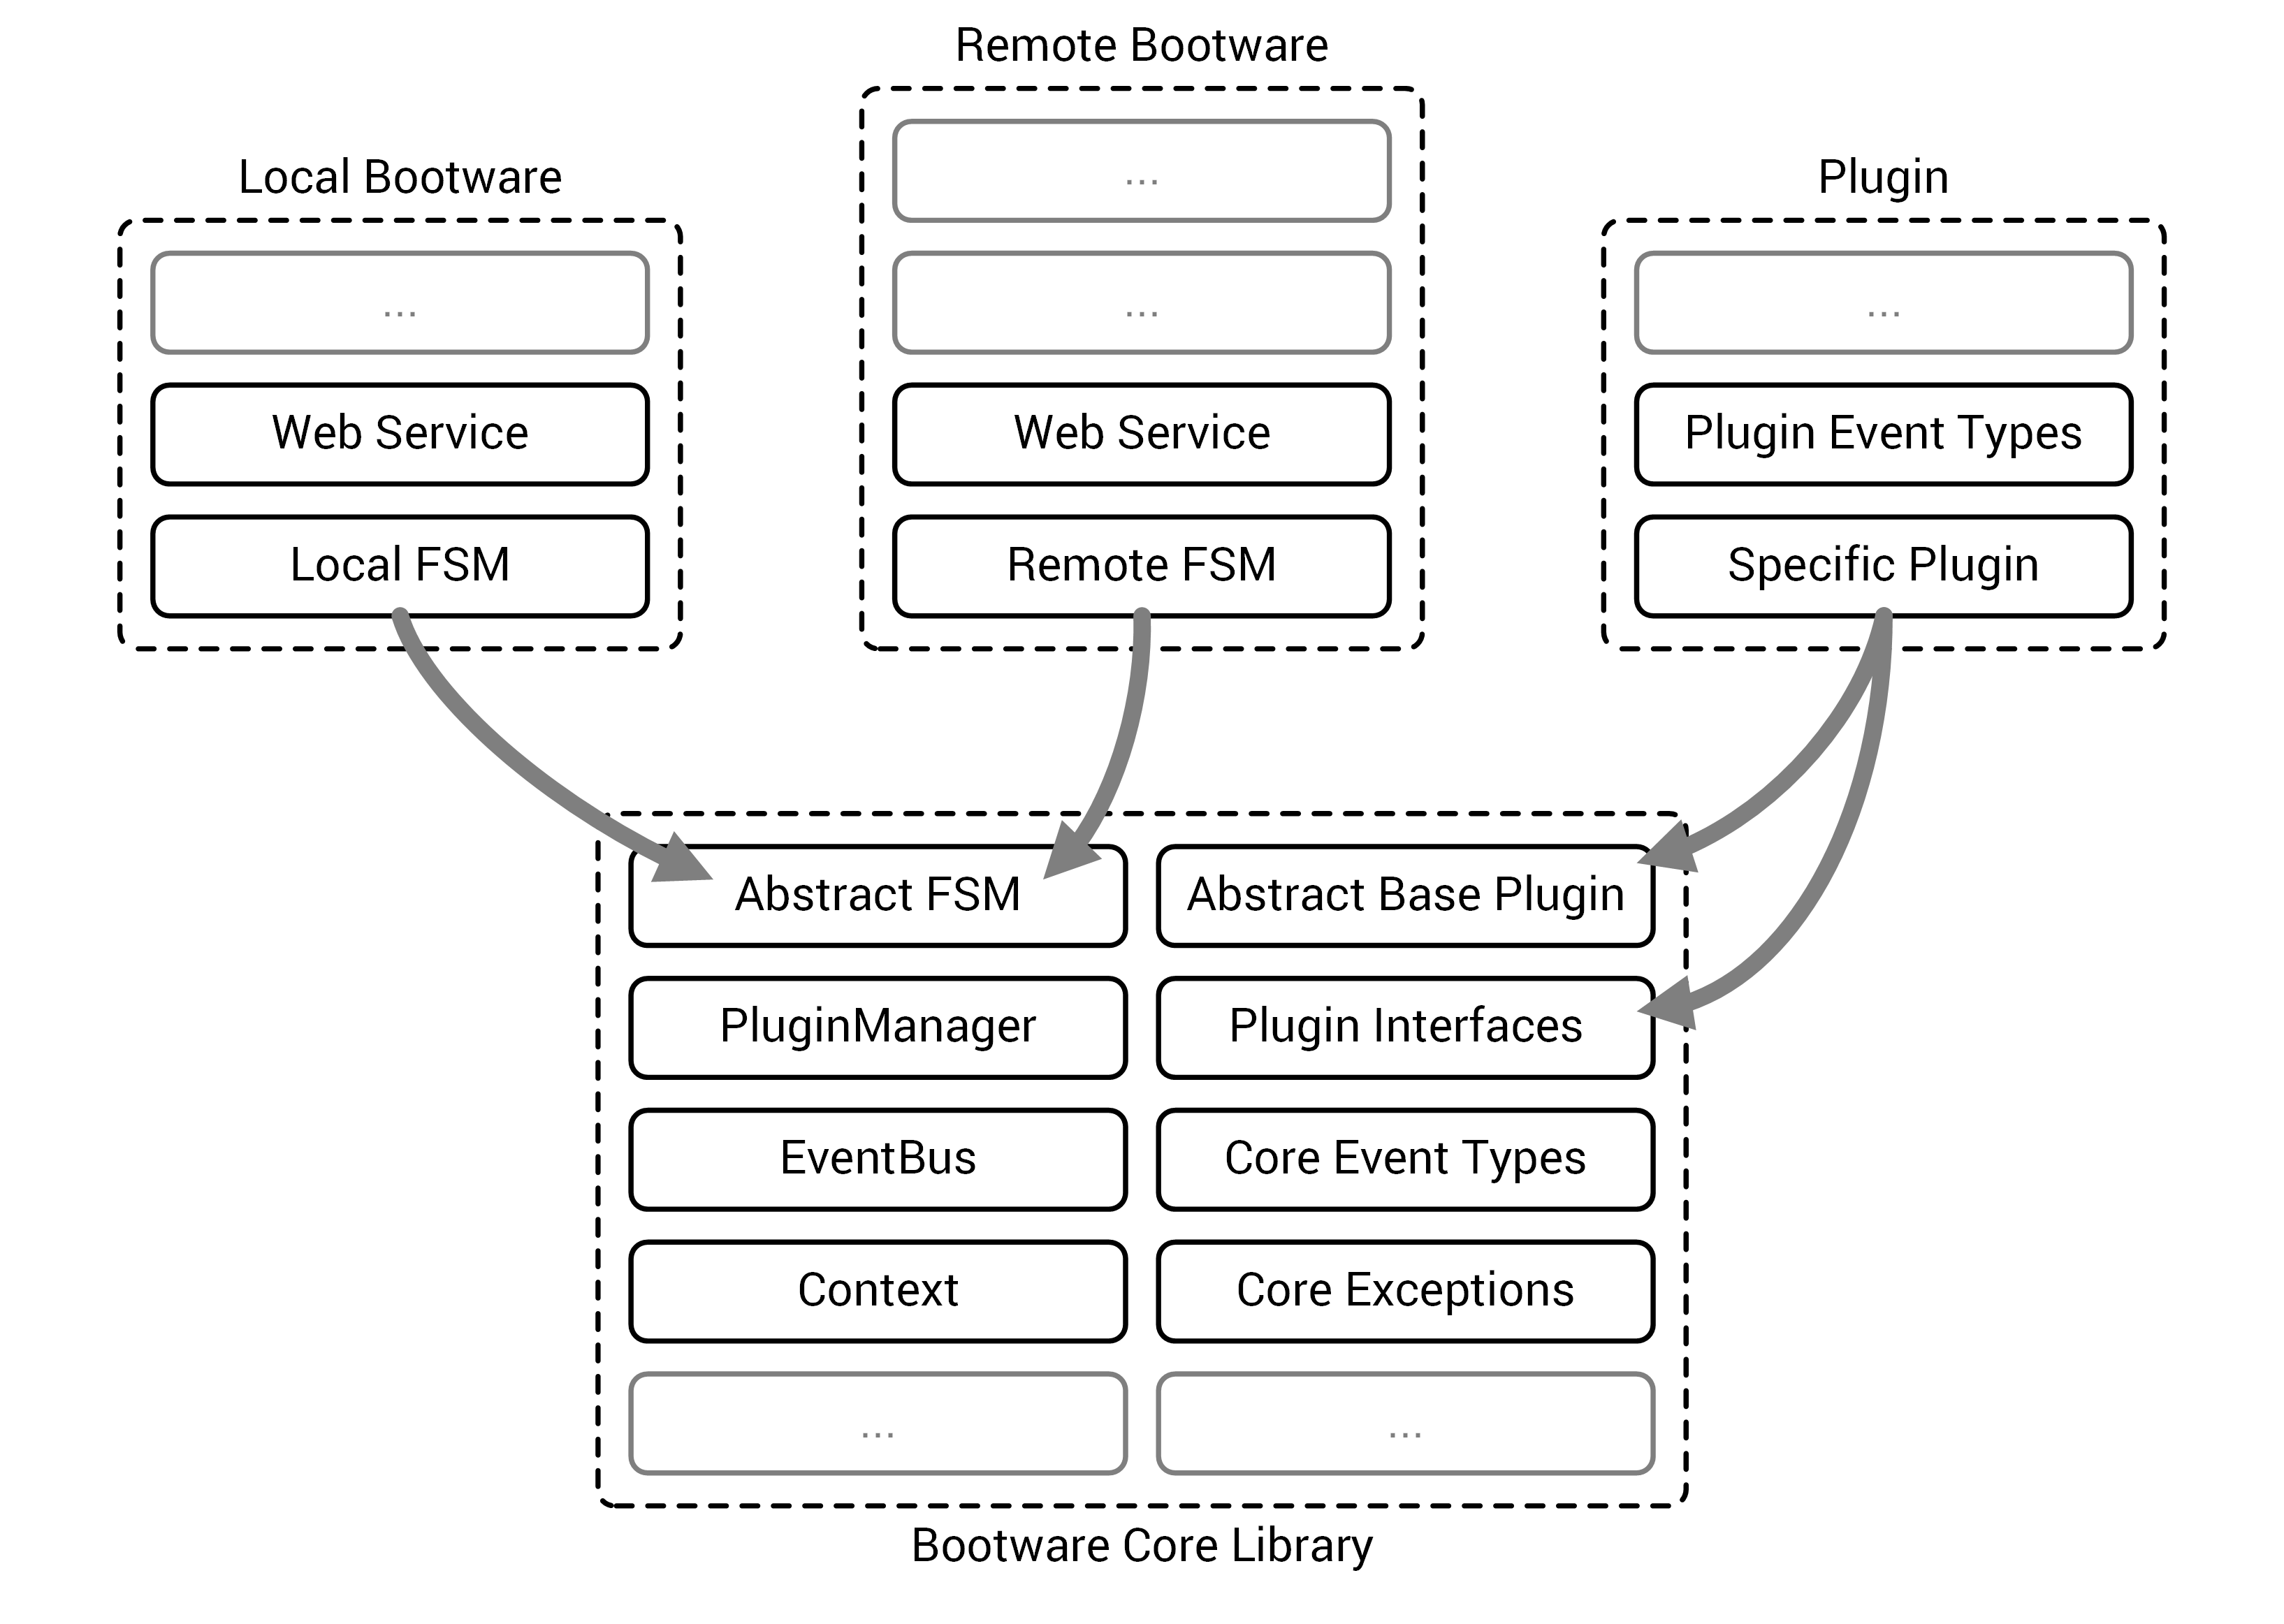
\includegraphics[resolution=600]{implementation/assets/core_library}
	\caption{The bootware core library and exemplary usage.}
	\label{image:corelibrary}
\end{figure}

Since we are using Java for the implementation, the core library will be a \textit{.jar} file containing common classes that will be imported by the local and remote bootware implementations and also by plugin implementations.
\autoref{image:corelibrary} shows a schematic view of the bootware core library and how its classes are used by various components.
We can see that the library includes an abstract FSM class, which is used by both the local and the remote bootware implementation.
The abstract FSM class defines common state machine functionality that is used by both bootware components.
This includes function definitions for the shared states shown in \autoref{image:flow_local} and \autoref{image:flow_remote}.
This way, the local and remote bootware can import shared states from the library and only have to define their custom states (e.g. the provision middleware states in the remote bootware or the send to remote state in the local bootware) and the state transitions.
They can also overwrite the states imported from the library if this is necessary.

The library also includes an abstract base plugin class, which implements some functionality that is common to all plugin.
Actual plugin implementations can extend this base plugin class to inherit this common functionality.
They also have to implement one of the plugin interfaces defined in the bootware core library, so for example, an infrastructure plugin has to implement the infrastructure plugin interface.

Aside from the code imported from the bootware core library, the components using the library are free to add various other code to their implementation.
This way, the remote bootware could implement some extra functionality not needed in the local bootware, or a plugin could define its own event types.


\section{Selecting Frameworks and Libraries}
\label{selecting}

Before we can begin with the actual implementation of the local and remote bootware, we have to decide on which frameworks and libraries we will use to implement the requested functionality.
In this section we present the frameworks and libraries we chose and the reasoning behind it.
We begin with plugin frameworks, followed by PubSub and FSM libraries.

\subsection{Plugin Frameworks}
\label{implementation:selecting:pluginframeworks}

All of the frameworks that we compare here offer the basic functionality that we need to extend the core bootware component, i.e. the developer defines interfaces that then are implemented by one or more plugins.
These plugins are compiled separately from the main component and are then packaged in \textit{.jar} files for distribution.
These packages are loaded during runtime and provide the implementation for the specific interface they implement.
There are however some advanced functional differences and some non-functional differences that will be considered here.

Dynamic loading allows us to load and replace plugins during runtime, without completely restarting the application.
This is an important feature, since it is possible that the bootware has to use many different plugins during its lifetime.
For example, this would be the case when several services have to be provisioned, each with different provisioning engines.
In this case, the bootware has to load the appropriate plugins for every provisioning engine to be able to fulfill its task.
We could of course just load every plugin at startup, switch between them internally when necessary, and never unload them.
This could become a problem if the number of available plugins increases in the future.
Then, loading all plugins could take some time and slow down the entire bootware process.
In many cases, some or most of the plugins would never be used and loading them wouldn't be necessary at all.
Therefore, it seems far more reasonable to load and unload plugins dynamically when needed.

Security is also a must have feature.
Consider the following scenario: The bootware component is used by multiple separate users who can share plugins using a plugin repository.
A malicious user could create a new plugin and upload it to the repository.
This plugin can contain virtually any code.
For example, it could erase all files or open a back door in the system when it is executed.
Other users might trust the plugin author and try the plugin without checking its code first.
Proper security feature might be able to prevent harm in such situations.
Due to time restrictions, plugin security will not be discussed further in this thesis, but it's still vital to select the right framework now, so that security features can be implemented in the future.

We also consider some non-functional features that might influence the selection.
There is already a plugin framework in use in the SimTech project, so it could be beneficial to choose the same framework, because the necessary knowledge and experience already exists.
The requirements section also mentioned that using software based on open standards is encouraged.
If possible, the complexity should be low while still providing all the necessary functional properties.
Frameworks with high popularity and an active development community might be more mature or provide more documentation and support.

\vspace*{\baselineskip}
\begingroup
	\centering
	\captionsetup{type=table}
	\begin{tabu}[!htbp]{rl|[0.5pt]cccc}

		&
		& \multicolumn{4}{c}{\textit{Plugin Frameworks}} \\[10pt]

		&
		& \begin{sideways} \textbf{SPI\footnote{\url{http://docs.oracle.com/javase/6/docs/api/java/util/ServiceLoader.html}\label{spi}}} \end{sideways}
		& \begin{sideways} \textbf{JSPF\footnote{\url{https://code.google.com/p/jspf}\label{jspf}}} \end{sideways}
		& \begin{sideways} \textbf{JPF\footnote{\url{http://jpf.sourceforge.net}\label{jpf}}} \end{sideways}
		& \begin{sideways} \textbf{OSGi\footnote{\url{http://www.osgi.org}\label{osgi}}} \end{sideways} \\

		\tabucline[0.5pt]{2-6}

		% NO  = \ding{55}
		% YES = \ding{51}

		\multirow{2}{*}{\textit{functional}}

		& \textbf{Dynamic Loading}
		& \ding{55}    % spi
		& \ding{55}    % jspf
		& \ding{51}    % jpf
		& \ding{51} \\ % osgi

		& \textbf{Security}
		& \ding{55}    % spi
		& \ding{55}    % jspf
		& \ding{55}    % jpf
		& \ding{51} \\ % osgi

		\tabucline[0.5pt]{2-6}

		\multirow{5}{*}{\textit{non-functional}}

		& \textbf{Used in SimTech}
		& \ding{55}    % spi
		& \ding{55}    % jspf
		& \ding{55}    % jpf
		& \ding{51} \\ % osgi


		& \textbf{Standard}
		& \textbf{(}\ding{51}\textbf{)} % spi
		& \ding{55}    % jspf
		& \ding{55}    % jpf
		& \ding{51} \\ % osgi

		& \textbf{Complexity}
		& low     % spi
		& low     % jspf
		& medium  % jpf
		& high \\ % osgi

		& \textbf{Popularity}
		& medium  % spi
		& low     % jspf
		& medium  % jpf
		& high \\ % osgi

		& \textbf{Active Development}
		& \ding{51}    % spi
		& \ding{55}    % jspf
		& \ding{55}    % jpf
		& \ding{51} \\ % osgi

		\tabucline[0.5pt]{2-6}

	\end{tabu}
	\caption{Feature comparison of Java plugin frameworks}
	\label{table:plugin_comparison}
\endgroup

\autoref{table:plugin_comparison} shows a comparison of four Java plugin frameworks, the first of which is the \nom{Service Provider Interface}{SPI}\footnote{\url{http://docs.oracle.com/javase/6/docs/api/java/util/ServiceLoader.html}}.
It is an extension mechanism integrated in Java which is a little more advanced then the manual extension mechanism described in \autoref{design:extensibility}.
It is also based on a set of interfaces and abstract classes that have to be implemented by an extension.
In the case of SPI, these interfaces and abstract classes are called services and a specific implementation of such a service is called service provider.
However, unlike in the manual approach, specific implementations are loaded from .jar files in specific directories or in the class path.
These .jar files also include metadata to identify the different service providers.

SPI is easy to use, doesn't depend on any external libraries, is well documented, and mature, since it is used in the \nom{Java Runtime Environment}{JRE}.
One could also say that it is somewhat standardized, since it is part of Java.
But as we can see in \autoref{table:plugin_comparison} on the left, it neither supports dynamic loading, nor security features and is therefore not a good fit for our needs.

The next contender is the \nom{Java Simple Plugin Framework}{JSPF}\footref{jspf}, an open-source plugin framework build for small to medium sized projects.
Its main focus is simplicity and the author explicitly states that it is not intended to replace JPF or OSGi\footnote{\url{https://code.google.com/p/jspf/wiki/FAQ}}.
As a result it is lightweight and easy to use but does not support advanced features like dynamic loading or security.

\nom{Java Plugin Framework}{JPF}\footref{jpf} is another open-source plugin framework.
Compared to JSPF it's a little more complex and popular.
As we can see in \autoref{table:plugin_comparison}, it also supports dynamic loading.
However, the last version was released in 2007 and development seems to have stopped.
This is not necessarily bad but might show that there will be no future development of this framework.

This leaves us with the final contender, which is \nom{Open Service Gateway initiative}{OSGi}\footref{osgi}, a plugin framework standard developed by the OSGi Alliance.
It provides a general-purpose Java framework that supports the deployment of extensible bundles~\autocite{osgi:spec}.
The right column of \autoref{table:plugin_comparison} shows, that it supports dynamic loading, as well as security.
OSGi is under active development, fairly popular, and has also been used in the SimTech project.
Compared to the other alternatives it is pretty complex, but considering the other factors, it is the only real alternative.
Therefore we will use OSGi to provide the extensibility required for the bootware.

Since OSGi by itself is only a standard, we still have to select an OSGI implementation.
As with all other libraries and frameworks we use, we are looking for an open-source implementation, so we will ignore commercial OSGi implementations.
There are three open-source OSGi implementations to choose from: Apache Felix\footnote{\url{http://felix.apache.org}}, Eclipse Equinox\footnote{\url{http://eclipse.org/equinox}}, and Knopflerfish\footnote{\url{http://www.knopflerfish.org}}.
All of them are under active development and implement the OSGi core framework specification, as well as the OSGi security specification (among others).
We will be using Apache Felix, since it is already being used in the SimTech project.
But it should be straight forward to change to another implementation in the future if necessary, since they all implement the same specification and should therefore in theory be completely interchangeable.

\subsection{PubSub Libraries}

Many of the well know Messaging Middlewares offer support for PubSub, for example ActiveMQ\footnote{\url{http://activemq.apache.org}}, RabbitMQ\footnote{\url{http://www.rabbitmq.com}}, and ZeroMQ\footnote{\url{http://zeromq.org}}.
But, since we are looking for an internal communication mechanism only, all of these solutions are somewhat overpowered.
We don't have to worry about network problems, so we don't need guaranteed delivery or message queuing capabilities.
We also don't need persistence or transactional capabilities
We don't have to handle millions of subscribers or events, so high scalability isn't a concern.
We don't even necessarily need asynchronous communication.
Instead, we need a lightweight in-memory solution.
Therefor we will ignore the middleware heavyweights and look for smaller, more light weight PubSub libraries.

\vspace*{\baselineskip}
\begingroup
	\centering
	\captionsetup{type=table}
	\begin{tabu}[!htbp]{rl|[0.5pt]ccccc}

		&
		& \multicolumn{5}{c}{\textit{PubSub Libraries}} \\[10pt]

		&
		& \begin{sideways} \textbf{MBassador\footnote{\url{https://github.com/bennidi/mbassador}\label{mbassasor}}} \end{sideways}
		& \begin{sideways} \textbf{Guava Event Bus\footnote{\url{https://code.google.com/p/guava-libraries/wiki/EventBusExplained}\label{guava}}} \end{sideways}
		& \begin{sideways} \textbf{Simple Java Event Bus\footnote{\url{https://code.google.com/p/simpleeventbus/}\label{simpleeventbus}}} \end{sideways}
		& \begin{sideways} \textbf{EventBus\footnote{\url{http://eventbus.org/}\label{eventbus}}} \end{sideways}
		& \begin{sideways} \textbf{Mycila PubSub\footnote{\url{https://github.com/mycila/pubsub}\label{mycilapubsub}}} \end{sideways} \\

		\tabucline[0.5pt]{2-7}

		% NO  = \ding{55}
		% YES = \ding{51}

		\multirow{6}{*}{\textit{Features}}

		& \textbf{Synchronous Invocation}
		& \ding{51}    % mbassador
		& \ding{51}    % guava
		& \ding{51}    % simpleeventbus
		& \ding{51}    % eventbus
		& \ding{51} \\ % mycila

		& \textbf{Asynchronous Invocation}
		& \ding{51}    % mbassador
		& \ding{51}    % guava
		& \ding{52}    % simpleeventbus
		& \ding{51}    % eventbus
		& \ding{51} \\ % mycila

		& \textbf{Filtering}
		& \ding{51}    % mbassador
		& \ding{55}    % guava
		& \ding{51}    % simpleeventbus
		& \ding{51}    % eventbus
		& \ding{55} \\ % mycila

		& \textbf{Event Hierarchy}
		& \ding{51}    % mbassador
		& \ding{51}    % guava
		& ?            % simpleeventbus
		& ?            % eventbus
		& \ding{51} \\ % mycila

		& \textbf{Prioritization}
		& \ding{51}    % mbassador
		& \ding{55}    % guava
		& \ding{55}    % simpleeventbus
		& \ding{51}    % eventbus
		& \ding{55} \\ % mycila

		& \textbf{Weak References}
		& \ding{51}    % mbassador
		& \ding{55}    % guava
		& \ding{51}    % simpleeventbus
		& \ding{51}    % eventbus
		& \ding{51} \\ % mycila

		\tabucline[0.5pt]{2-7}

		\multirow{3}{*}{\textit{non-functional}}

		& \textbf{Popularity}
		& medium % mbassador
		& medium % guava
		& low    % simpleeventbus
		& high   % eventbus
		& low \\ % mycila

		& \textbf{Maturity}
		& medium % mbassador
		& medium % guava
		& low    % simpleeventbus
		& high   % eventbus
		& low \\ % mycila

		& \textbf{Documentation}
		& medium % mbassador
		& medium % guava
		& low    % simpleeventbus
		& high   % eventbus
		& low \\ % mycila

		\tabucline[0.5pt]{2-7}

	\end{tabu}
	\caption{Feature comparison of Java PubSub libraries}
	\label{table:pubsub_comparison}
\endgroup

\section{State Machine Libraries}
\label{implementation:selecting:statemachine}

Since we want to implement the bootware process as a finite state machine, we must now decide how we will do it.
It would certainly be possible to go with a hand made state machine implementation, but the time for this thesis is limited and we should use it for the actual design of the bootware.
Therefore, it would be better to use an existing state machine library.
In general, we are looking for an event-driven FSM, which allows us to define a set of states and transition between those states when specific events occur.
Ideally we would prefer a standardized way to define the FSM and avoid proprietary formats.
But we also don't want the FSM to be overly complex to use.
\autoref{table:statemachine_comparison} shows six state machine libraries available for Java.

\vspace*{\baselineskip}
\begingroup
	\centering
	\captionsetup{type=table}
	\begin{tabu}[!htbp]{rX[2l]|[0.5pt]X[c]X[c]X[c]X[c]X[c]X[c]}

		&
		& \multicolumn{6}{c}{\textit{State Machine Libraries}} \\[10pt]

		&
		& \begin{sideways} \textbf{Commons SCXML\footnote{\url{http://commons.apache.org/proper/commons-scxml/}\label{scxml}}} \end{sideways}
		& \begin{sideways} \textbf{EasyFlow\footnote{\url{https://github.com/Beh01der/EasyFlow}\label{easyflow}}} \end{sideways}
		& \begin{sideways} \textbf{SMC\footnote{\url{http://smc.sourceforge.net/}\label{smc}}} \end{sideways}
		& \begin{sideways} \textbf{stateless4j\footnote{\url{https://github.com/oxo42/stateless4j/}\label{stateless4j}}} \end{sideways}
		& \begin{sideways} \textbf{squirrel-foundation\footnote{\url{https://github.com/hekailiang/squirrel}\label{squirrel}}} \end{sideways}
		& \begin{sideways} \textbf{Unimod\footnote{\url{http://unimod.sourceforge.net/}\label{unimod}}} \end{sideways} \\

		\tabucline[0.5pt]{2-8}

		% NO  = \ding{55}
		% YES = \ding{51}

		\multirow{2}{*}{\begin{sideways}\textit{functional}\end{sideways}}

		& \textbf{Event Driven}
		& \ding{51}    % scxml
		& \ding{51}    % easyflow
		& \ding{51}    % smc
		& \ding{51}    % stateless4j
		& \ding{51}    % squirrel
		& \ding{51} \\ % unimod


		& \textbf{Description \linebreak Language}
		& SCXML                  % scxml
		& Java                   % easyflow
		& .sm                    % smc
		& Java                   % stateless4j
		& Java, SCXML            % squirrel
		& UML, \linebreak XML \\ % unimod

		\tabucline[0.5pt]{2-8}

		\multirow{4}{*}{\begin{sideways}\textit{non-func.}\end{sideways}}

		& \textbf{Complexity}
		& med.    % scxml
		& low    % easyflow
		& med.    % smc
		& low    % stateless4j
		& low    % squirrel
		& high \\ % unimod

		& \textbf{Popularity}
		& med.    % scxml
		& low       % easyflow
		& med.    % smc
		& low       % stateless4j
		& med.    % squirrel
		& med. \\ % unimod

		& \textbf{Maturity}
		& low     % scxml
		& med.  % easyflow
		& high    % smc
		& med.  % stateless4j
		& med.  % squirrel
		& high \\ % unimod

		& \textbf{Documentation}
		& med.  % scxml
		& low     % easyflow
		& high    % smc
		& low     % stateless4j
		& high    % squirrel
		& high \\ % unimod

		\tabucline[0.5pt]{2-8}

	\end{tabu}
	\caption{Feature comparison of Java state machine libraries.}
	\label{table:statemachine_comparison}
\endgroup

Apache Commons SCXML\footref{scxml} aims to be an java state machine engine that is capable of executing state machines defined as \nom{State Chart XML}{SCXML}.
SCXML is a working draft specification for a general-purpose event-based state machine language that is currently being developed by the \nom{World Wide Web Consortium}{W3C}\autocite{scxml}.
Apache Commons SCXML looks like a good match for our needs, since it is event-based and also using a (soon to be) standard.
But the current state of the implementation seems to be lacking since the SCXML specification has changed a lot.
The most recent release is version 0.9, which was released in late 2008.
It is to be replaced by version 2.0 that is currently being worked on and includes major changes, but a release date is not yet in sight~\autocite{scxml:roadmap}.

EasyFlow\footref{easyflow} is a simple and lightweight FSM for Java.
It is event-driven, but only supports describing the FSM directly in Java code.
Compared to the other alternatives, it is not very well documented and not very popular.
It would however be able to do the job.

\nom{State Machine Compiler}{SMC}\footref{smc} is a state machine compiler that targets fifteen different programming languages, including Java.
It generates FSMs from a definition in \textit{.sm} files.
SMC is mature and has good documentation, but the use of an extra definition language and the extra step of compiling it into a Java representation seems to be to complicated for our needs.

Stateless4j\footref{stateless4j} is a lightweight library for creating FSMs directly in Java code.
Compared to the other alternatives, it lacks in documentation and doesn't seem to be very popular.

Squirrel-foundation\footref{squirrel} is a lightweight, flexible, and extensible FSM library for Java.
Although relatively new, it is feature rich, well documented and relatively popular.
It also supports some advanced features that might be useful.
For example, it supports SCXML import and export.

Unimod\footref{unimod} is a project that can create FSMs from UML descriptions created by an eclipse plugin.
Unlike the other alternative, Unimod aims to create a unified methodology for application development and not just a library.
This seems to be to complex for our needs.


\section{Context}
\label{implementation:context}

\vspace*{\baselineskip}
\begin{listing}[!htbp]
	\inputminted[
		label=context.xml,
		frame=topline,
		linenos,
		frame=lines,
		tabsize=2,
		framesep=0.3cm,
		fontsize=\small
	]{xml}{implementation/assets/context.xml}
	\caption{Sample context represented in XML.}
	\label{lst:context:sample}
\end{listing}

\autoref{lst:context:sample} shows an exemplary context in XML form.
As we can see in line 2-4, it is required to define the infrastructure, connection, and payload plugins that should be used during the bootstrapping process by supplying the name of the plugin \textit{.jar}.
It is also possible to specify a provision workflow middleware plugin, as can be seen in line 6-8.
This is optional and will only be used on the first request, when the remote bootware will also call a provisioning engine to provision the workflow middleware.
This is also where the package reference in line 10 will be used, which points to the workflow middleware package that should be provisioned by the provisioning engine called by the provision workflow middleware plugin.
In line 12-28 we can also see the optional configuration list.
If it is supplied in the context, it will override configuration values with the same name in the default configuration list that can be set with the setConfiguration operation.
If it is not supplied, the default configuration will be used.

\section{Web Service Interface}
\label{implementation:webservice}

In \autoref{design:communication} we decided to use web service calls and returns as external communication mechanism and in \autoref{design:context} we decided to pass along a context.
Now, we need to the define the interface that will be made available by the web service to the outside.
We obviously need the two main operations, deploy and undeploy, to be available from the outside.
In \autoref{design:context} we also described the \textit{setConfiguration} operation that has to be supported.

\subsection{Deploy}

The \textit{deploy} operation will be called by at least two different components.
Once by the bootware modeler plugin to deploy the remote bootware and the workflow middleware, and then each time the provisioning manager needs to provision a new service during a workflow execution.
\autoref{lst:webservice:deployrequest} shows an exemplary deploy request as soap message.
In line 6 we can see that the deploy method is called with the context provided as argument in line 7-11.
In this particular example, only the required plugins are specified, which could be a call from the provisioning manager.

\vspace*{\baselineskip}
\begin{listing}[!htbp]
	\inputminted[
		label=deploy-request.xml,
		frame=topline,
		linenos,
		frame=lines,
		tabsize=2,
		framesep=0.3cm,
		fontsize=\small
	]{xml}{implementation/assets/deploy-request.xml}
	\caption{Sample deploy request in a soap message.}
	\label{lst:webservice:deployrequest}
\end{listing}

The response that is return once the request has been executed successfully is shown in \autoref{lst:webservice:deployresponse}.
It contains a list of endpoint references in line 5-10, which contains a reference to the payload that was deployed during the request, in this case OpenTOSCA.

\vspace*{\baselineskip}
\begin{listing}[!htbp]
	\inputminted[
		label=deploy-response.xml,
		frame=topline,
		linenos,
		frame=lines,
		tabsize=2,
		framesep=0.3cm,
		fontsize=\small
	]{xml}{implementation/assets/deploy-response.xml}
	\caption{Sample deploy response in a soap message.}
	\label{lst:webservice:deployresponse}
\end{listing}

If the deploy request somehow failed, a soap message containing a soap fault will be returned, which is shown in \autoref{lst:webservice:deployerror}.
It contains a fault string with an error description in line 5, as well as the original DeployException that was thrown by the deploy operation in line 7-10.

\vspace*{\baselineskip}
\begin{listing}[!htbp]
	\inputminted[
		label=deploy-error.xml,
		frame=topline,
		linenos,
		frame=lines,
		tabsize=2,
		framesep=0.3cm,
		fontsize=\small
	]{xml}{implementation/assets/deploy-error.xml}
	\caption{Sample deploy error in a soap message.}
	\label{lst:webservice:deployerror}
\end{listing}

\subsection{Undeploy}

Like the \textit{deploy} operation, the \textit{undeploy} operation will be called by multiple components to reverse the actions that where previously made by deploy operations.
\autoref{lst:webservice:undeployrequest} shows an exemplary undeploy request in a soap message.
As argument it contains one or more endpoint references to already deployed payloads, as can be seen in line 7-12.

\vspace*{\baselineskip}
\begin{listing}[!htbp]
	\inputminted[
		label=undeploy-request.xml,
		frame=topline,
		linenos,
		frame=lines,
		tabsize=2,
		framesep=0.3cm,
		fontsize=\small
	]{xml}{implementation/assets/undeploy-request.xml}
	\caption{Sample undeploy request in a soap message.}
	\label{lst:webservice:undeployrequest}
\end{listing}

When all payloads have been undeployed successfully, a response will be send, as shown in \autoref{lst:webservice:undeployresponse}.
The response is empty since there is nothing interesting to return.

\vspace*{\baselineskip}
\begin{listing}[!htbp]
	\inputminted[
		label=undeploy-response.xml,
		frame=topline,
		linenos,
		frame=lines,
		tabsize=2,
		framesep=0.3cm,
		fontsize=\small
	]{xml}{implementation/assets/undeploy-response.xml}
	\caption{Sample undeploy response in a soap message.}
	\label{lst:webservice:undeployresponse}
\end{listing}

In case of a failure, an error will be return.
As can be seen in \autoref{lst:webservice:undeployerror}, it has the same layout as the error returned by the deploy operation.
It contains a soap fault string in line 5 and the original UndeployException thrown by the undeploy operation in line 7-10.

\vspace*{\baselineskip}
\begin{listing}[!htbp]
	\inputminted[
		label=undeploy-error.xml,
		frame=topline,
		linenos,
		frame=lines,
		tabsize=2,
		framesep=0.3cm,
		fontsize=\small
	]{xml}{implementation/assets/undeploy-error.xml}
	\caption{Sample undeploy error in a soap message.}
	\label{lst:webservice:undeployerror}
\end{listing}

\subsection{SetConfiguration}

In addition to the main deploy and undeploy operations, the bootware web service also supports the \textit{setConfiguration} operation.
Using this operation, the configuration can be set independently from deploy requests if necessary.
\autoref{lst:webservice:setconfigurationrequest} shows an exemplary setConfiguration request.
In line 7-23, it contains a configuration list, which can contain one or more configuration sets.
Each configuration set is made up of one or more configuration entries, which are key value pairs, where the key describes the configuration type and the value the actual configuration value.
What content a particular key has to contain depends on what the plugins are looking for when they read the configuration.
In the example code in line 9, we send one configuration set for AWS, which consists of two credentials, a secret key in line 12-15 and an accessKey in line 16-19.

\vspace*{\baselineskip}
\begin{listing}[!htbp]
	\inputminted[
		label=setConfiguration-request.xml,
		frame=topline,
		linenos,
		frame=lines,
		tabsize=2,
		framesep=0.3cm,
		fontsize=\small
	]{xml}{implementation/assets/setConfiguration-request.xml}
	\caption{Sample setConfiguration request in a soap message.}
	\label{lst:webservice:setconfigurationrequest}
\end{listing}

If the setConfiguration operation was successful, the response in \autoref{lst:webservice:setconfigurationresponse} will be returned.
Again, it is empty, since there is nothing interesting to return.

\vspace*{\baselineskip}
\begin{listing}[!htbp]
	\inputminted[
		label=setConfiguration-response.xml,
		frame=topline,
		linenos,
		frame=lines,
		tabsize=2,
		framesep=0.3cm,
		fontsize=\small
	]{xml}{implementation/assets/setConfiguration-response.xml}
	\caption{Sample setConfiguration response in a soap message.}
	\label{lst:webservice:setconfigurationresponse}
\end{listing}

Like the deploy and undeploy operations, the setConfiguration operation also returns an error message if the operation failed.
As can be seen in \autoref{lst:webservice:setconfigurationerror}, it also contains a soap fault string in line 5 and the original SetConfigurationException thrown by the setConfiguration operation in line 7-10.

\vspace*{\baselineskip}
\begin{listing}[!htbp]
	\inputminted[
		label=setConfiguration-error.xml,
		frame=topline,
		linenos,
		frame=lines,
		tabsize=2,
		framesep=0.3cm,
		fontsize=\small
	]{xml}{implementation/assets/setConfiguration-error.xml}
	\caption{Sample setConfiguration error in a soap message.}
	\label{lst:webservice:setconfigurationerror}
\end{listing}

\subsection{Shutdown}

The shutdown operation triggers the shutdown procedure.
During this procedure, all active payloads will be undeployed.
The local bootware will also forward this request to the remote bootware and wait for a response so that it can deprovision the remote bootware before shutting down itself.
\autoref{lst:webservice:shutdownrequest} shows a shutdown request in a SOAP message.
No parameters are required.

\vspace*{\baselineskip}
\begin{listing}[!htbp]
	\inputminted[
		label=shutdown-request.xml,
		frame=topline,
		linenos,
		frame=lines,
		tabsize=2,
		framesep=0.3cm,
		fontsize=\small
	]{xml}{implementation/assets/shutdown-request.xml}
	\caption{Sample shutdown request in a soap message.}
	\label{lst:webservice:shutdownrequest}
\end{listing}

If the additional processes executed during shutdown (i.e. undeploy payloads or middleware) were successful, the response in \autoref{lst:webservice:shutdownresponse} will be returned.

\vspace*{\baselineskip}
\begin{listing}[!htbp]
	\inputminted[
		label=shutdown-response.xml,
		frame=topline,
		linenos,
		frame=lines,
		tabsize=2,
		framesep=0.3cm,
		fontsize=\small
	]{xml}{implementation/assets/shutdown-response.xml}
	\caption{Sample shutdown response in a soap message.}
	\label{lst:webservice:shutdownresponse}
\end{listing}

If the additional processes failed for some reason, an error response like the one shown in \autoref{lst:webservice:shutdownerror} will be returned.
It contains a soap fault string in line 5 and the original ShutdownException thrown by the shutdown operation in line 7-10.

\vspace*{\baselineskip}
\begin{listing}[!htbp]
	\inputminted[
		label=shutdown-error.xml,
		frame=topline,
		linenos,
		frame=lines,
		tabsize=2,
		framesep=0.3cm,
		fontsize=\small
	]{xml}{implementation/assets/shutdown-error.xml}
	\caption{Sample shutdown error in a soap message.}
	\label{lst:webservice:shutdownerror}
\end{listing}

\section{Plugin Types}
\label{design:plugins}

We can already tell from the requirements that we must at least support two different plugin types, one for different cloud providers and one for different provisioning engines.
The former are required because we may want to provision into different cloud environments.
The latter are required because we might want to use different provisioning engines to do so.

The cloud provider plugins will be responsible for creating and removing resources in cloud environments and making them available for the user to configure and use.
This could be bare bone VMs (like AWS EC2 instances), or PaaS environments (like AWS Beanstalk).
We do not even have to constrain these plugins to cloud resources and can make them more abstract, as long as we can run the plugin and get an IP address to a computer resource that we can use.
For example, we could also provide a plugin that starts and stops VMs on our local machine, which could be useful for quick and inexpensive local testing.
So a better name for these plugins would be \textit{infrastructure plugins}.

The same line of thinking can be used on the provisioning engine plugins.
All that we care about is that we can get some software running on a given infrastructure and that we get back an URL where we can find this software once it is up and running.
A better name for these plugins would therefore be \textit{application plugins}.

Now that we have infrastructure plugins and application plugins, we should be able to provision the infrastructure we need and use application plugins to install and run any software on it.
But there is a step in between provisioning the infrastructure and installing the software that we are glancing over: We have to somehow communicate with the infrastructure to be able to install something on it.
The communication functionality could be part of either the infrastructure plugins or the application plugins, or it could be separated into independent communication plugins.

For the sake of efficiency and extensibility it would be best to use independent communication plugins.
For example, if a user wanted to add a new communication type that should be used to install x applications in y environments, they could do so by writing one new communication plugin, instead of adding the functionality x-times to all application plugins, or y-times to all infrastructure plugins.
This would also reduce code duplication.
Therefore, a third plugin type is necessary: The \textit{communication plugins}.

The remote bootware also has to handle the initial provisioning of the workflow middleware, which involves calling a provisioning engine to tell it to start the provisioning process.
Because this has to be done differently for all provisioning engines, it would make sense to also package this functionality into plugins that can be interchanged.
We therefore introduce a fourth plugin type: The \textit{provision workflow middleware plugins}.

In \autoref{design:communication} we also introduced the notion of secondary communication channels realized by plugins.
We can generalize this into a more versatile fifth plugin type: The \textit{event plugins}.
These plugins are a bit less specific than the four other types.
They allow users to add functionality that reacts to (or creates) events inside the bootware.
How the actual event system will be implemented will be discussed in \autoref{design:internalcomm}.
With this fifth plugin type we have now covered all plugin types we will need.
We will describe each plugin type in more detail, but before we do this, we will describe the common operations that all plugin types have to implement.

\vspace*{\baselineskip}
\begingroup
	\centering
	\captionsetup{type=table}
	\renewcommand{\arraystretch}{2}
	\begin{tabu}[!htbp]{X[2,r]X[2,c]X[2,c]X[6,l]}

			\multicolumn{1}{c}{\textbf{Operation}}
		& \multicolumn{1}{c}{\textbf{Input}}
		& \multicolumn{1}{c}{\textbf{Output}}
		& \multicolumn{1}{c}{\textbf{Description}} \\

		\tabucline[0.5pt]{1-4}

			initialize
		& Configuration
		& -
		& Is called by the plugin manager when the plugin is loaded \\

			shutdown
		& -
		& -
		& Is called by the plugin manager when the plugin is unloaded \\

	\end{tabu}
	\caption{Common operations to be implemented by all plugin types.}
	\label{table:all_plugins}
\endgroup

\autoref{table:all_plugins} shows the two common operations that all plugin types must implement.
The initialize operation is called by the plugin manager when it loads a plugin.
This operation can be used by plugin authors to initialize the plugin, for example by creating internal objects that will be used by other plugin operations later on.
It takes a configuration object as parameter, which is taken from the request context.
This allows the plugins to be configured from the outside if necessary.
The shutdown operation is called by the plugin manager when it unloads a plugin.
It can be useful to clean up plugin resources before the plugin is removed, for example by deleting temporary files or closing a communication channel.

\subsection{Infrastructure Plugins}

Infrastructure plugins are responsible for provisioning any infrastructure that the user wants to use during the bootware process.
This could be VMs on a local machine, or IaaS or PaaS environments in the cloud.
To be able to do this, an infrastructure plugin has to implement a range of functions using some API or SDK provided by the virtualization software or cloud provider.

\autoref{table:infra_plugins} shows the operations a plugins of this type should implement.
The deploy operation is responsible for deploying a resource and getting it to a state, where a connection to the resource can be established using a communication plugin.
It takes no input parameters, but relies on the configuration passed to the initialize operation to get the configuration details it needs, like login credentials.
If the deployment was successful, it returns an instance object, which contains information about the created instance, such as its IP address and login information.

The undeploy operation removes a resource that was previously deployed using the deploy operation.
In case of a local VM this could mean that it stops the running VM.
In case of a cloud resource this could mean that it completely removes the resource so that no further costs are incurred.
As input it takes an instance object created earlier by the deploy operation.

\vspace*{\baselineskip}
\begingroup
	\centering
	\captionsetup{type=table}
	\renewcommand{\arraystretch}{2}
	\begin{tabu}[!htbp]{X[2,r]X[2,c]X[2,c]X[6,l]}

			\multicolumn{1}{c}{\textbf{Operation}}
		& \multicolumn{1}{c}{\textbf{Input}}
		& \multicolumn{1}{c}{\textbf{Output}}
		& \multicolumn{1}{c}{\textbf{Description}} \\

		\tabucline[0.5pt]{1-4}

			deploy
		& -
		& Instance
		& Deploys a communication ready instance of some resource and returns an instance object \\

			undeploy
		& Instance
		& -
		& Completely removes a given instance \\

	\end{tabu}
	\caption{Interface to be implemented by infrastructure plugins.}
	\label{table:infra_plugins}
\endgroup

\subsection{Communication Plugins}

Communication plugins are responsible for creating a communication channel to previously deployed resources that can later be used by application plugins to execute their operations on the resource.
The connection could be made by using SSH, \nom{remote desktop connection}{RDC}, \nom{virtual private network}{VPN}, Telnet, or other communication mechanisms supported by the resource.
The communication plugins should be implemented generically, so that they can be used for all kinds of resources.

\autoref{table:conn_plugins} shows the operations that this type of plugin has to implement.
The connect operation establishes a connection to a specific resource.
The resource is specified by the instance object that is passed as input to the connect operation.
If the connection was established successfully, the operation returns a connection object that can be used later by application plugins to execute operations through this connection.
The disconnect operation closes a connection that was previously established by the connect operation.
As input, it takes a connection object that was previously created by the connect operation.

\vspace*{\baselineskip}
\begingroup
	\centering
	\captionsetup{type=table}
	\renewcommand{\arraystretch}{2}
	\begin{tabu}[!htbp]{X[2,r]X[2,c]X[2,c]X[6,l]}

			\multicolumn{1}{c}{\textbf{Operation}}
		& \multicolumn{1}{c}{\textbf{Input}}
		& \multicolumn{1}{c}{\textbf{Output}}
		& \multicolumn{1}{c}{\textbf{Description}} \\

		\tabucline[0.5pt]{1-4}

			connect
		& Instance
		& Connection
		& Establishes a connection to the given instance\\

			disconnect
		& Connection
		& -
		& Disconnects a given connection \\

	\end{tabu}
	\caption{Interface to be implemented by communication plugins.}
	\label{table:conn_plugins}
\endgroup

\subsection{Application Plugins}

Application plugins are responsible for installing, uninstalling, starting, and stopping software on an infrastructure instance.
This process can include the uploading of files and the execution of remote commands on an instance.

\autoref{table:payload_plugins} shows the operations that plugins of this type should implement.
The deploy operation installs an application on an instance.
This can include uploading files from the local machine or downloading files from other machines.
To execute this operation, a connection to the instance is necessary, which is supplied as input with the connection object.
The undeploy operation removes an application from an instance.
In most cases this will not be necessary, because the instance will be destroyed in the undeploy phase and with it all the application data (assuming it was not stored in some other persistent storage).
This method is provided for completeness and for special cases.
The start operation starts an application which previously was installed with the deploy operation.
If the application was started successfully, it returns the URL to the running application.
The stop operation stops the execution of a previously started application.
In most cases this will not be necessary, because the application will be removed together with the instance in the undeploy phase.
This method is provided for completeness and for special cases.

\vspace*{\baselineskip}
\begingroup
	\centering
	\captionsetup{type=table}
	\renewcommand{\arraystretch}{2}
	\begin{tabu}[!htbp]{X[2,r]X[2,c]X[2,c]X[6,l]}

			\multicolumn{1}{c}{\textbf{Operation}}
		& \multicolumn{1}{c}{\textbf{Input}}
		& \multicolumn{1}{c}{\textbf{Output}}
		& \multicolumn{1}{c}{\textbf{Description}} \\

		\tabucline[0.5pt]{1-4}

			deploy
		& Connection
		& -
		& Deploys the application over the given connection\\

			undeploy
		& Connection
		& -
		& Undeploys the application over the given connection\\

			start
		& Connection
		& URL
		& Starts the application over the given connection\\

			stop
		& Connection
		& -
		& Stops the application over the given connection\\

	\end{tabu}
	\caption{Interface to be implemented by application plugins.}
	\label{table:payload_plugins}
\endgroup

\subsection{Provision Workflow Middleware Plugins}

Provision workflow middleware plugins provide the bootware with a unified way to call provisioning engines and trigger provisioning and deprovisioning operations.
\autoref{table:provisioningengine_plugins} shows the operations that these plugins should implement.
The provision operation calls a provisioning engine and trigger the provisioning process.
It takes two inputs: An endpoint reference, which points to the provisioning engine that should be used, and a package reference, which points to the workflow middleware package that the provisioning engine should provision.
When completed successfully, the provisioning operation returns a list of information about to the just provisioned workflow middleware.
This list can contain arbitrary information, such as a URL pointing to the workflow middleware or any other information that might be necessary to connect the modeler to the workflow middleware.
The deprovision operation calls a provisioning engine and triggers the deprovisioning process.
It takes the same inputs as the provisioning operation, an endpoint reference to the provisioning engine and a package reference.

\vspace*{\baselineskip}
\begingroup
	\centering
	\captionsetup{type=table}
	\renewcommand{\arraystretch}{2}
	\begin{tabu}[!htbp]{X[2,r]X[2,c]X[2,c]X[6,l]}

			\multicolumn{1}{c}{\textbf{Operation}}
		& \multicolumn{1}{c}{\textbf{Input}}
		& \multicolumn{1}{c}{\textbf{Output}}
		& \multicolumn{1}{c}{\textbf{Description}} \\

		\tabucline[0.5pt]{1-4}

			provision
		& Endpoint Reference, Package Reference
		& Information List
		& Tells the provisioning engine to provision the given workflow middleware package\\

			deprovision
		& Endpoint Reference, Package Package
		& -
		& Tells the provisioning engine to deprovision the given workflow middleware package\\

	\end{tabu}
	\caption{Interface to be implemented by provision workflow middleware plugins.}
	\label{table:provisioningengine_plugins}
\endgroup

In parallel to this diploma thesis, another diploma thesis is being written about the provisioning manager, which will also use plugins to call provisioning engines~\autocite{nedim}.
Because these plugins are similar in functionality, it makes sense to create libraries for particular provisioning engines that can then be used by both the provisioning manager plugins and the bootware plugins.
This would reduce overall code duplication.
We will not describe those libraries in more detail in this thesis.
We assume that such libraries will exist and that we can use them for implementing our plugins.

\subsection{Event Plugins}

Apart from the initialize and shutdown operations described in \autoref{table:all_plugins}, event plugins only implement the handle operation, as shown in \autoref{table:event_plugins}.
It takes an event type as input.
Every time an event of this type is triggered, all handle operation associated with this event type will be called and can execute some code, for example logging the event.
Note that each event plugin can declare more than one handle function to be able to react to multiple events.

\vspace*{\baselineskip}
\begingroup
	\centering
	\captionsetup{type=table}
	\renewcommand{\arraystretch}{2}
	\begin{tabu}[!htbp]{X[2,r]X[2,c]X[2,c]X[6,l]}

			\multicolumn{1}{c}{\textbf{Operation}}
		& \multicolumn{1}{c}{\textbf{Input}}
		& \multicolumn{1}{c}{\textbf{Output}}
		& \multicolumn{1}{c}{\textbf{Description}} \\

		\tabucline[0.5pt]{1-4}

			handle
		& Event Type
		& -
		& Is called every time an event of the given type is triggered\\

	\end{tabu}
	\caption{Interface to be implemented by event plugins.}
	\label{table:event_plugins}
\endgroup

